\section{Randomized Shellsort}

Randomized Shellsort~\citeA{RandShellSort} is a randomized data-oblivious sorting algorithm notable for its ability to sort data with very high probability, using only $\Theta(n \log n)$ comparisons.

The algorithm itself is fairly simplistic, consisting entirely of applications of a special region comparison function, whose method of operation will be described shortly. This can then optionally be followed by clean-up phase entirely constructed from already known data-oblivious sorting algorithms.

It is especially important to note that the size and location of regions being compared will be entirely dependent on the size of the data, and that matchings between elements is determined randomly with no knowledge of the input.

The analysis showing the low failure rate of the algorithm is unfortunately rather lengthy, and somewhat complex, but can be found in~\citeA{RandShellSort}.

\subsection{Region Comparison}
\label{sec:RegionCompare}

The comparison between regions is done by computing a random matching between elements of the two regions, and performing a \texttt{Compare-Exchange} operation between each pair of matched indices.
This procedure will be repeated $c$ times to perform a full comparison of regions.~\citeA{RandShellSort} shows that when $c \geq 4$ the full region comparison will have properties closely related to those of \textepsilon -halvers.

The pseudo-code for the region comparison is shown in Algorithm~\ref{RegionCompare}.

For a graphical representation of the region comparison, see Figure~\ref{fig:CompareExchange}.


\begin{algorithm}
\caption{Region Compare}\label{RegionCompare}
\begin{algorithmic}[1]
	\Statex $A$: Array input of \texttt{Compare-Exchange} compatible elements
	\Statex $i$: Index of first region
	\Statex $j$: Index of second region
	\Statex $size$: Size of regions to compare
\Procedure{RegionCompare}{$A, i, j, size$}
\For{$1 \dots c$}
	\Comment $c$ is a predetermined constant
	\State $matching \gets \mathtt{shuffle}([0 \dots size-1])$
	\For{$k = 0 \dots size-1$}
		\State $\mathtt{Compare\mbox{-}Exchange}(A, i + k, j + matching[k])$
	\EndFor
\EndFor
\EndProcedure
\end{algorithmic}
\end{algorithm}

\begin{figure}
\center
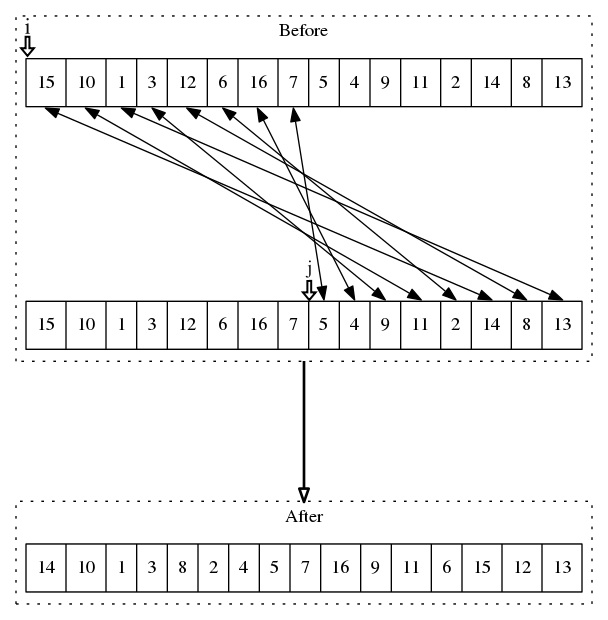
\includegraphics[width=\textwidth]{Graphics/regcmp.png}
\caption{Region Compare with $c=1$ of size 8 on 16 elements of data. $i$ and $j$ are the first and last halves of the shown arrays respectively. Note that the \emph{Before} region shows the matching with the same array.}
\label{fig:CompareExchange}
\end{figure}

\subsection{The Main Algorithm}

Having constructed the region comparison operation, we move on to the main algorithm.

The important part of Randomized Shellsort consist of applying the region comparison on the input data in ever decreasing region sizes, starting at $n/2$, and halving in size until they reach $1$. Note that there will be only $\log(n)$ such region sizes, and that $n$ is assumed to be a non-trivial power of 2.

For each region size, six different runs through the data are performed. These runs fall into two distinct groups, a \emph{shaker} phase and a \emph{brick} phase.

In the \emph{shaker} phase we run through the regions, comparing them with the next region in ascending order, and then do the same for descending order. This resembles the variant of Shellsort called Shaker Sort~\citeA{ShakerSort}, and is intended to quickly move misplaced elements to the correct end of the input.

The \emph{brick} phase will first run through the regions comparing them to the regions $3$ places further up, then a run comparing $2$ places up, and then finally it will perform runs comparing first the even regions with their next neighbour, and then the odd regions with their next neighbour.
This somewhat resembles the Brick Sort mentioned in~\citeB{ShellsortRelated}, and it is important for the analysis that this sequence of comparisons creates a complete 4-tournament of any 4 adjacent regions.
This phase serves the purpose of moving elements short distances among nearby regions of the input. 

Finally, following the main part of the algorithm, a clean-up step is taken to move a polylogarithmic amount of stray elements into place.~\citeA{RandShellSort} notes that this can be done by repeated applications of Pratt's variant of Shellsort~\citeA{PrattThesis}, but states that this final clean-up step is most likely needed only as an artefact from the analysis of the sorting probability.

It is fairly easy to see that if we can perform the region comparison in linear time, then the main algorithm will perform $\Theta(n \log n)$ operations. Using the region comparison of Section~\ref{sec:RegionCompare}, we can easily guarantee linear time region comparisons, leading to the desired running time. 

Given this sequence of region comparisons, and the \texttt{RegionCompare} procedure from Algorith~\ref{RegionCompare}, it is clearly seen that the Randomized Shellsort will perform at most $5cn\log n$ comparisons in addition to the clean-up phase, which is low compared to the huge constants of~\citeA{AKS}, if $c$ is kept at a reasonable level.

The exact structure of the algorithm is best described in pseudo-code, as seen in Algorithm~\ref{RandomizedShellsort}.

\begin{algorithm}
\caption{Randomized Shellsort}\label{RandomizedShellsort}
\begin{algorithmic}[1]
	\Statex $A$: Array input of \texttt{Compare-Exchange} compatible elements
	\Statex $n$: Size of $A$
\Procedure{RandomizedShellsort}{$A, n$}
\For{$jump = n/2, n/4, n/8 \dots 1$}
	\For{$i = 0 \dots n/jump-2$}
	\Comment Shaker pass part 1
		\State $\mathtt{RegionCompare}(A, i\cdot jump, (i+1)\cdot jump, jump)$
	\EndFor
	\For{$i = n/jump-1 \dots 1$}
	\Comment Shaker pass part 2
		\State $\mathtt{RegionCompare}(A, (i-1)\cdot jump, i\cdot jump, jump)$
	\EndFor
	\For{$i = 0 \dots n/jump-4$}
	\Comment Brick pass part 1
		\State $\mathtt{RegionCompare}(A, i\cdot jump, (i+3)\cdot jump, jump)$
	\EndFor
	\For{$i = 0 \dots n/jump-3$}
	\Comment Brick pass part 2
		\State $\mathtt{RegionCompare}(A, i\cdot jump, (i+2)\cdot jump, jump)$
	\EndFor
	\For{$i = 0, 2, 4 \dots n/jump-2$}
	\Comment Brick pass part 3
		\State $\mathtt{RegionCompare}(A, i\cdot jump, (i+1)\cdot jump, jump)$
	\EndFor
	\For{$i = 1, 3, 5 \dots n/jump-3$}
	\Comment Brick pass part 4
		\State $\mathtt{RegionCompare}(A, i \cdot jump, (i+1)\cdot jump, jump)$
	\EndFor
\EndFor
\State $\mathtt{Clean-Up(A)}$
\EndProcedure
\end{algorithmic}
\end{algorithm}
